\documentclass{beamer}
%\documentclass[handout]{beamer}

%\setbeamertemplate{theorems}[numbered]
\setbeamertemplate{theorems}[ams style]
\setbeamertemplate{caption}[numbered]

\usepackage{lmodern} % get rid of warnings
\usepackage{caption} % improved spacing between figure and caption

\DeclareCaptionLabelSeparator{horse}{:\quad} % change according to your needs
\captionsetup{
	labelsep = horse,
	figureposition = bottom
} 

%\usepackage[utf8]{inputenc}
\usepackage[T1]{fontenc}
\usepackage[english]{babel}

\usepackage{amsfonts}
\usepackage{amsmath}
\usepackage{amssymb}
\usepackage{amsthm}
% \usepackage[frenchstyle]{mathalpha}
% \usepackage[OMLmathsfit]{isomath}
\usepackage{graphicx}
\usepackage{color} % for ps_tex inclusions
\usepackage{fmtcount} % th, e.g. \ordinalnum{4}
\usepackage{algorithm, algorithmic} % algorithms
\usepackage{tikz}
\usetikzlibrary{bayesnet,calc,tikzmark}
\usetikzlibrary{shapes.geometric}
\usepackage{multimedia}
\usepackage{xr}
\usepackage{hyperref}
\externaldocument[notes-]{notes}
\usetheme{Madrid}
\usecolortheme{seagull}

\newcommand{\itb}{\item[$\bullet$]}
\newcommand{\dps}{\displaystyle}

\def\<{{\guillemotleft}}
\def\>{{\guillemotright}}

\def\vs1{\vspace{1mm}}
\def\v3{\vspace{3mm}}

\newcommand{\II}{\,\mbox{I\hskip -0.600em 1}}

\newcommand{\BSX}{{\boldsymbol X}}
\newcommand{\BSY}{{\boldsymbol Y}}
\newcommand{\BSZ}{{\boldsymbol Z}}

\newcommand{\bsx}{{\boldsymbol x}}
\newcommand{\bsy}{{\boldsymbol y}}
\newcommand{\bsz}{{\boldsymbol z}}

\newcommand{\bsalpha}{{\boldsymbol \alpha}}

\newcommand{\MA}{{\mathcal A}}
\newcommand{\MB}{{\mathcal B}}
\newcommand{\MC}{{\mathcal C}}
\newcommand{\MD}{{\mathcal D}}
\newcommand{\ME}{{\mathcal E}}
\newcommand{\MF}{{\mathcal F}}
\newcommand{\MG}{{\mathcal G}}
\newcommand{\MK}{{\mathcal K}}
\newcommand{\MM}{{\mathcal M}}
\newcommand{\MN}{{\mathcal N}}
\newcommand{\MO}{{\mathcal O}}
\newcommand{\MQ}{{\mathcal Q}}
\newcommand{\MS}{{\mathcal S}}
\newcommand{\MT}{{\mathcal T}}
\newcommand{\MU}{{\mathcal U}}
\newcommand{\MV}{{\mathcal V}}
\newcommand{\MX}{{\mathcal X}}

\newcommand{\TY}{{\tilde Y}}

\newcommand{\NN}{\ensuremath{\mathbb{N}}}
\newcommand{\RR}{\ensuremath{\mathbb{R}}}

\newcommand{\card}{\mbox{card}}
\newcommand{\pa}{\mbox{pa}}

\newcommand{\De}{\mbox{De}}
\newcommand{\Nd}{\mbox{Nd}}
\newcommand{\Ne}{\mbox{Ne}}

\newcommand{\indep}{\perp\!\!\!\perp}
\newcommand{\condindep}[3]{#1 \indep #2 \vert #3}
\newcommand{\condindepP}[4]{#1 \indep_{#4} #2 \vert #3}
\newcommand{\ts}[3]{#1_{#2}^{#3}}
\newcommand{\set}[1]{\{#1\}}

\newcommand{\myth}[1]{#1^{\mbox{\scriptsize{th}}}}


\newcommand{\myarray}[2]{\left(\begin{array}{#1}#2\end{array}\right)}

\title{Learning Probabilities and Causality}

\subtitle{Chapter V - Linear dynamical systems (LDS)} % (optional)

\author[Xavi]{Xavier Alameda-Pineda}
% - Use the \inst{?} command only if the authors have different
%   affiliation.

\institute{}

\date{}

\makeatother
\setbeamertemplate{footline}
{
  \leavevmode%
%   \hbox{%
%   \begin{beamercolorbox}[wd=.4\paperwidth,ht=2.25ex,dp=1ex,center]{author in head/foot}%
%     \usebeamerfont{author in head/foot}\insertshortauthor
%   \end{beamercolorbox}%
%   \begin{beamercolorbox}[wd=.6\paperwidth,ht=2.25ex,dp=1ex,center]{title in head/foot}%
    \usebeamerfont{title in head/foot}\hfill
    \insertframenumber{} / \inserttotalframenumber\hspace*{1ex}
%   \end{beamercolorbox}}%
%   \vskip0pt%
}
\makeatletter
\setbeamertemplate{navigation symbols}{}

\AtBeginSection[]{
  \begin{frame}
  \vfill
  \centering
  \begin{beamercolorbox}[sep=8pt,center,shadow=true,rounded=true]{title}
    \usebeamerfont{title}\insertsectionhead\par%
  \end{beamercolorbox}
  \vfill
  \end{frame}
}

\AtBeginSubsection[]{
  \begin{frame}
  \vfill
  \centering
  \begin{beamercolorbox}[sep=8pt,center,shadow=true,rounded=true]{title}
    \usebeamerfont{title}\insertsectionhead\\---\\\insertsubsectionhead\par%
  \end{beamercolorbox}
  \vfill
  \end{frame}
}

\date{}

\newcommand{\bs}[1]{\boldsymbol{#1}}

\newcommand{\exercise}[2]{\noindent\colorbox{blue!10}{\parbox{0.995\textwidth}{\textbf{Exercise \ref{notes-ex:#1}}: #2}}\\}
\newcommand{\remark}[2]{\noindent\colorbox{red!10}{\parbox{0.995\textwidth}{\textbf{Remark \ref{notes-rmk:#1}}: #2}}\\}

\newcommand{\oncolor}[2]{\only<#1>{\color{#2}}}

\definecolor{mygreen}{rgb}{0,0.75,0}
\definecolor{myred}{rgb}{0.75,0,0}
\definecolor{myblue}{rgb}{0,0,0.9}
\newcommand{\paint}[2]{{\color{#1}#2}}

\newcommand{\expectation}[2][]{%
\ifthenelse { \equal {#1} {} }%
% Expectation w/o distribution
{\mathbb{E}\left\{#2\right\}}%
% Expectation with distribution
{\mathbb{E}_{#1}\left\{#2\right\}}
}

%%%%%%%%%%%%%%%%%%%%%%%%%%%%%%%%%%%%%%%%%%%%%%%%%%%%%%%%%%%%%%

\begin{document}

\begin{frame}
    \titlepage
    \vspace{-1.9cm}
\end{frame}

\begin{frame}{Outline}
 \tableofcontents
\end{frame}

% \begin{frame}{Practical issues}
%   Instead of the shared overleaf document, we propose to allow\\ \textbf{2 double-sided hand-written A4 paper sheets}.\vspace{1cm}
%   
%   These notes should help you remember things, because we do not want you to learn by heart.\vspace{1cm}
%   
%   Instead, we would like you to learn how to use the various mathematical objects we've seen.
% \end{frame}


%%%%%%%%%%%%%%%%%%%%%%%%%%%%%%%%%%%%%%%%%%%%%%%%%%%%%%%%%%%%%%
\section{Introduction to LDS}
%%%%%%%%%%%%%%%%%%%%%%%%%%%%%%%%%%%%%%%%%%%%%%%%%%%%%%%%%%%%%%

%%%%%%%%%%%%%%%%%%%%%%%%%%%%%%%%%%%%%%%%%%%%%%%%%%%%%%%%%%%%%%
\begin{frame}{GMM}
 Hidden categorical variable:
 \begin{equation*} p(\bs{z}=k) = \pi_k \qquad k\in\{1,\ldots,K\},\end{equation*}
 Gaussian conditional observed variable:
 \begin{equation*} p(\bs{x}|\bs{z}=k) = {\cal N}(\bs{x};\bs{\mu}_k,\bs{\Sigma}_k).\end{equation*}
 EM algorithm on the observation set $\{\bs{x}_n\}_{n=1}^N$, compute and maxmise the \textit{complete-data expected log-likelihood}:
 \begin{equation*} Q(\bs{\Theta},\bs{\Theta}^{\textrm{old}}) =  \sum_{n=1}^N\mathbb{E}_{p(\bs{z}_n|\bs{x}_n,\bs{\Theta}^{\textrm{old}})} \log p(\bs{x}_n,\bs{z}_n;\bs{\Theta}).\end{equation*}
\end{frame}

%%%%%%%%%%%%%%%%%%%%%%%%%%%%%%%%%%%%%%%%%%%%%%%%%%%%%%%%%%%%%%
\begin{frame}{HMM}
 Hidden categorical variable with temporal links:
 \begin{equation*} p(\bs{z}_t=k|\bs{z}_{t-1}=j) = \tau_{jk} \qquad j,k\in\{1,\ldots,K\},\end{equation*}
 Gaussian conditional observed variable:
 \begin{equation*} p(\bs{x}_t|\bs{z}_t=k) = {\cal N}(\bs{x}_t;\bs{\mu}_k,\bs{\Sigma}_k).\end{equation*}
 EM algorithm on the observed sequence set $\{\bs{x}_n=(\bs{x}_{n1},\ldots,\bs{x}_{nT_n})\}_{n=1}^N$:
 \begin{equation*} Q(\bs{\Theta},\bs{\Theta}^{\textrm{old}}) =  \sum_{n=1}^N\mathbb{E}_{p(\bs{z}_n|\bs{x}_n,\bs{\Theta}^{\textrm{old}})} \log p(\bs{x}_n,\bs{z}_n;\bs{\Theta}).\end{equation*}
 The expression is the same, but now $\bs{x}_n$ and $\bs{z}_n$ are sequences.
\end{frame}

%%%%%%%%%%%%%%%%%%%%%%%%%%%%%%%%%%%%%%%%%%%%%%%%%%%%%%%%%%%%%%
\begin{frame}{PPCA}
Hidden continuous variable:
\begin{equation*} p(\bs{z}) = {\cal N}(\bs{z};0,I),\end{equation*}
Linear-Gaussian conditional model:
\begin{equation*} p(\bs{x}|\bs{z}) = {\cal N}(\bs{x};\bs{A}\bs{z}+\bs{b},\sigma^2 I).\end{equation*}
EM algorithm on the observation set $\{\bs{x}_n\}_{n=1}^N$:
\begin{equation*} Q(\bs{\Theta},\bs{\Theta}^{\textrm{old}}) =  \sum_{n=1}^N\mathbb{E}_{p(\bs{z}_n|\bs{x}_n,\bs{\Theta}^{\textrm{old}})} \log p(\bs{x}_n,\bs{z}_n;\bs{\Theta}).\end{equation*}
\end{frame}

%%%%%%%%%%%%%%%%%%%%%%%%%%%%%%%%%%%%%%%%%%%%%%%%%%%%%%%%%%%%%%
\begin{frame}{What else could we like to do?}
 \begin{center}
  \textbf{\large Let's watch a video!!!}
 \end{center}
\end{frame}


%%%%%%%%%%%%%%%%%%%%%%%%%%%%%%%%%%%%%%%%%%%%%%%%%%%%%%%%%%%%%%
\begin{frame}{What is missing?}
\begin{center}
\footnotesize
\begin{tabular}{c||c|c}
 ``$\bs{z}$'' & Discrete & Continuous \\\hline\hline
 No Temporal & {GMM $p(\bs{z}=k) = \pi_k$} & {PPCA $p(\bs{z}) = {\cal N}(\bs{z};0,I)$}\\\hline
 Temporal & {HMM $p(\bs{z}_t=k|\bs{z}_{t-1}=j) = \tau_{jk}$} & {\color{myred}{LDS} $p(\bs{z}_t|\bs{z}_{t-1}) = {\cal N}(\bs{z}_t;\bs{A}\bs{z}_{t-1},\bs{\Gamma})$}
\end{tabular}
\end{center}\vspace{3mm}

\pause


We are missing a model with a \textbf{sequence of continuous latent variables}.\vspace{3mm}

Other examples:\vspace{3mm}\\
\footnotesize
(i) Monitoring the temperature of a furnace (latent) with an external sensor (observed).\\
(ii) Estimating a plane's trajectory (latent) from radar measures (observed).\\
(iii) Tracking the position of a person (latent) from the direction of the voice (observed).\vspace{3mm}

\normalsize
Things we can do:\vspace{3mm}\\
\footnotesize
(i) Filtering: use causal (non-future) obs, to estimate present latent.\\
(ii) Smoothing: use all obs. to estimate all latents.\\
(iii) Predicting: use causal obs. to estimate future latent.\vspace{3mm}


% Let's watch a video!

% These are the so-called \textbf{linear dynamical systems}:
% \begin{equation*}
%  p(\bs{z}_1) = {\cal N}(\bs{z}_1;\bs{d},\bs{\Omega}) \qquad p(\bs{z}_t|\bs{z}_{t-1}) = {\cal N}(\bs{z}_t;\bs{A}\bs{z}_{t-1},\bs{\Gamma}),
%  \end{equation*}
%  \begin{equation*}
%  p(\bs{x}_t|\bs{z}_t) = {\cal N}(\bs{x}_t;\bs{C}\bs{z}_t,\bs{\Sigma}).
% \end{equation*}
\end{frame}

%%%%%%%%%%%%%%%%%%%%%%%%%%%%%%%%%%%%%%%%%%%%%%%%%%%%%%%%%%%%%%
\begin{frame}{The linear dynamical system (LDS) model (I)}
\begin{columns}
 \begin{column}{0.7\textwidth}
  Sequence of latent variables $(\bs{z}_t)_{t=1}^T$, $\bs{z}_t\in\mathbb{R}^{d_z}$.\\
  Sequence of observations $(\bs{x}_t)_{t=1}^T$, $\bs{x}_t\in\mathbb{R}^{d_x}$.
 \end{column}
 \begin{column}{0.3\textwidth}
  \begin{figure}
    \scalebox{0.7}{
    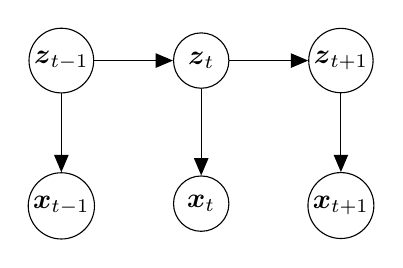
\begin{tikzpicture}
    \node[latent] (zm) {$\bs{z}_{t-1}$};
    \node[latent,right=of zm] (z) {$\bs{z}_t$};
    \node[latent,right=of z] (zp) {$\bs{z}_{t+1}$};
    \node[latent,below=of zm] (xm) {$\bs{x}_{t-1}$};
    \node[latent,below=of z,yshift=-1mm] (x) {$\bs{x}_t$};
    \node[latent,below=of zp] (xp) {$\bs{x}_{t+1}$};
    \edge{zm} {xm,z};
    \edge{z} {x,zp};
    \edge{zp} {xp};
    \end{tikzpicture}}
  \end{figure}
 \end{column}
\end{columns}
First order dependency on the latent variables:
\begin{align*}
 p(\bs{x}_{1:T},\bs{z}_{1:T}) &= p(\bs{x}_{1:T}|\bs{z}_{1:T})p(\bs{z}_{1:T}) \\ &= \prod_{t=1}^T p(\bs{x}_t|\bs{z}_t) \prod_{t=2}^T p(\bs{z}_t|\bs{z}_{t-1}) p(\bs{z}_1).
\end{align*}
The dependencies are the same as in the HMM model. The latent variables, and therefore their distributions, are different.
\end{frame}

%%%%%%%%%%%%%%%%%%%%%%%%%%%%%%%%%%%%%%%%%%%%%%%%%%%%%%%%%%%%%%
\begin{frame}{The linear dynamical system (LDS) model (II)}
\begin{columns}
 \begin{column}{0.7\textwidth}
  \begin{align*}
 p(\bs{x}_{1:T},\bs{z}_{1:T}) &= \prod_{t=1}^T p(\bs{x}_t|\bs{z}_t) \prod_{t=2}^T p(\bs{z}_t|\bs{z}_{t-1}) p(\bs{z}_1).
\end{align*}\end{column}
 \begin{column}{0.3\textwidth}
  \begin{figure}
    \scalebox{0.7}{
    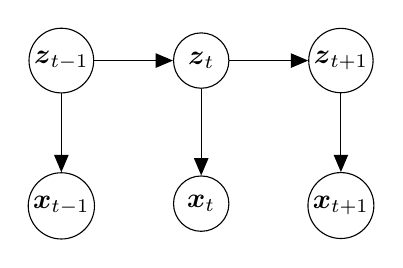
\begin{tikzpicture}
    \node[latent] (zm) {$\bs{z}_{t-1}$};
    \node[latent,right=of zm] (z) {$\bs{z}_t$};
    \node[latent,right=of z] (zp) {$\bs{z}_{t+1}$};
    \node[latent,below=of zm] (xm) {$\bs{x}_{t-1}$};
    \node[latent,below=of z,yshift=-1mm] (x) {$\bs{x}_t$};
    \node[latent,below=of zp] (xp) {$\bs{x}_{t+1}$};
    \edge{zm} {xm,z};
    \edge{z} {x,zp};
    \edge{zp} {xp};
    \end{tikzpicture}}
  \end{figure}
 \end{column}
\end{columns}\vspace{3mm}

 \begin{equation*}
 p(\bs{x}_t|\bs{z}_t) = {\cal N}(\bs{x}_t;\bs{C}\bs{z}_t,\bs{\Sigma}).
\end{equation*}
\begin{equation*}
 p(\bs{z}_1) = {\cal N}(\bs{z}_1;\bs{d},\bs{\Omega}) \qquad p(\bs{z}_t|\bs{z}_{t-1}) = {\cal N}(\bs{z}_t;\bs{A}\bs{z}_{t-1},\bs{\Gamma}),
 \end{equation*}

How many \textbf{free} parameters has the model? {\footnotesize ($\bs{x}_t\in\mathbb{R}^{d_x}$, $\bs{z}_t\in\mathbb{R}^{d_z}$)}\\\vspace{2mm}
\only<1>{$\bs{d}$, $\bs{A}$, $\bs{C}$?}\pause
$\bs{d}\rightarrow d_z$, $\bs{A}\rightarrow d_z^2$, $\bs{C}\rightarrow d_xd_z$\\\only<2>{$\bs{\Omega}$, $\bs{\Gamma}$, $\bs{\Sigma}$?}\pause
$\bs{\Omega}\rightarrow d_z(d_z+1)/2$, $\bs{\Gamma}\rightarrow d_z(d_z+1)/2$, and 
$\bs{\Sigma}\rightarrow d_x(d_x+1)/2$.\\\vspace{3mm}
{\small $\bs{\Theta}=\{\bs{d},\bs{\Omega},\bs{A},\bs{\Gamma},\bs{C},\bs{\Sigma}\}$ are the model parameters. The parameters appearing in the next slides are \textbf{NOT} parameters of the model, but \textit{parameters of the EM}.}
\end{frame}

%%%%%%%%%%%%%%%%%%%%%%%%%%%%%%%%%%%%%%%%%%%%%%%%%%%%%%%%%%%%%%
\section{Multivariate Gaussian distribution (again)}
%%%%%%%%%%%%%%%%%%%%%%%%%%%%%%%%%%%%%%%%%%%%%%%%%%%%%%%%%%%%%%

%%%%%%%%%%%%%%%%%%%%%%%%%%%%%%%%%%%%%%%%%%%%%%%%%%%%%%%%%%%%%%
\begin{frame}{Preliminaries for the EM for LDS}
 Our objective is to derive the EM algorithm for LDS.\\\vspace{3mm}
 
 Before going through the EM, we will be discussing properties of the multivariate Gaussian distribution\\\vspace{3mm}
 
 We \textbf{forget for a while about the sequences} and consider now the concatenation of $\bs{x}$ and $\bs{z}$: $\bs{y} = [\bs{x}^\top,\bs{z}^\top]^\top$, $\bs{y}\in\mathbb{R}^{d_x+d_z}$.\\\vspace{3mm}
 
 We've seen that if $p(\bs{z})$ is a Gaussian, and $p(\bs{x}|\bs{z})$ is a linear-Gaussian, then the joint distribution on $\bs{y} = [\bs{x}^\top,\bs{z}^\top]^\top$ is a Gaussian as well. But is the opposite true?
\end{frame}

%%%%%%%%%%%%%%%%%%%%%%%%%%%%%%%%%%%%%%%%%%%%%%%%%%%%%%%%%%%%%%
\begin{frame}{Structured multivariate Gaussian distribution}
 If we write $p(\bs{y}) = \MN(\bs{y};\bs{\mu}_y,\bs{\Sigma}_{yy})$ then we can write:
 \begin{equation*}
  \bs{\mu}_{y}=\left(\begin{array}{c}\bs{\mu}_x\\\bs{\mu}_z\end{array}\right) \qquad
  \bs{\Sigma}_{yy}= \left(\begin{array}{cc} \bs{\Sigma}_{xx} & \bs{\Sigma}_{xz} \\ \bs{\Sigma}_{zx} & \bs{\Sigma}_{zz} \end{array}\right)
 \end{equation*}\vspace{3mm}
 
 We would like to derive properties of $p(\bs{z})$ and $p(\bs{x}|\bs{z})$ from $p(\bs{y})$.\pause

 In order to evaluate $\MN(\bs{y};\bs{\mu}_y,\bs{\Sigma}_{yy})$, we need to compute:
 \begin{equation*}
  \bs{\Sigma}_{yy}^{-1} = \left(\begin{array}{cc} \bs{\Sigma}_{xx} & \bs{\Sigma}_{xz} \\ \bs{\Sigma}_{zx} & \bs{\Sigma}_{zz} \end{array}\right)^{-1} \only<2>{=} {\only<3>{\color{myred}\neq} \left(\begin{array}{cc} \bs{\Sigma}_{xx}^{-1} & \bs{\Sigma}_{xz}^{-1} \\ \bs{\Sigma}_{zx}^{-1} & \bs{\Sigma}_{zz}^{-1} \end{array}\right)}
 \end{equation*}\vspace{3mm}\pause
 
 {\color{myred}\LARGE NOOOOOOOOOOOOOO!!!! TOTAL FAIL!!!}\vspace{3mm}\\
 
 Think about how do you invert a $2\times 2$ matrix, or what if $\bs{\Sigma}_{xy}$ is not square.
\end{frame}


%%%%%%%%%%%%%%%%%%%%%%%%%%%%%%%%%%%%%%%%%%%%%%%%%%%%%%%%%%%%%%
\begin{frame}{Block-inversion matrix}
\remark{block-wise-inversion}{There are two version of the block-wise inversion lemma:
\begin{equation*}
 \myarray{cc}{\bs{A} & \bs{B} \\ \bs{C} & \bs{D}}^{-1} = \myarray{cc}{\bs{M} & - \bs{M}\bs{B}\bs{D}^{-1} \\ -\bs{D}^{-1}\bs{C}\bs{M} & 
\bs{D}^{-1} + \bs{D}^{-1}\bs{C}\bs{M}\bs{B}\bs{D}^{-1}} \label{eq:block-inversion}
\end{equation*}
with $\bs{M} = (\bs{A}-\bs{B}\bs{D}^{-1}\bs{C})^{-1}$. And:
\begin{equation*}
 \myarray{cc}{\bs{A} & \bs{B} \\ \bs{C} & \bs{D}}^{-1} = \myarray{cc}{ \bs{A}^{-1} + \bs{A}^{-1}\bs{B}\bs{N}\bs{C}\bs{A}^{-1} & - \bs{A}^{-1}\bs{C}\bs{N} \\ -\bs{N}\bs{B}\bs{A}^{-1} & 
\bs{N}} \label{eq:block-inversion-v2}
\end{equation*}
with $\bs{N} = (\bs{D}-\bs{C}\bs{A}^{-1}\bs{B})^{-1}$.
}\vspace{3mm}

\exercise{block-wise-inversion}{Prove that both are indeed inverses of the original matrix. As a consequence they have to be equal. You will need the Woodbory lemma.}


\end{frame}


%%%%%%%%%%%%%%%%%%%%%%%%%%%%%%%%%%%%%%%%%%%%%%%%%%%%%%%%%%%%%%
\begin{frame}{The precision matrix}
 If we apply this to $p(\bs{y})$, the precision matrix $\bs{\Lambda}_{yy}$ (the inverse of $\bs{\Sigma}_{yy}$) is:
\begin{equation*}
 \bs{\Lambda}_{yy} =  \myarray{cc}{\bs{\Lambda}_{xx} & \bs{\Lambda}_{xz} \\ \bs{\Lambda}_{zx} & \bs{\Lambda}_{zz}} = \myarray{cc}{\bs{\Lambda}_{xx} & 
-\bs{\Lambda}_{xx}\bs{\Sigma}_{xz}\bs{\Sigma}_{zz}^{-1} \\ -\bs{\Sigma}_{zz}^{-1}\bs{\Sigma}_{zx}\bs{\Lambda}_{xx} & \bs{\Sigma}_{zz}^{-1} + 
\bs{\Sigma}_{zz}^{-1}\bs{\Sigma}_{zx}\bs{\Lambda}_{xx}\bs{\Sigma}_{xz}\bs{\Sigma}_{zz}^{-1}}\label{eq:block-inversion-covariance}
\end{equation*}
with $\bs{\Lambda}_{xx} = (\bs{\Sigma}_{xx} - \bs{\Sigma}_{xz}\bs{\Sigma}_{zz}^{-1}\bs{\Sigma}_{zx})^{-1}$.\vspace{5mm}

Now, what can we now say about:
\begin{itemize}
 \item $p(\bs{z})$, and
 \item $p(\bs{x}|\bs{z})$?
\end{itemize}

\end{frame}

%%%%%%%%%%%%%%%%%%%%%%%%%%%%%%%%%%%%%%%%%%%%%%%%%%%%%%%%%%%%%%
\begin{frame}{The conditional and marginal distributions}
\exercise{conditional-structured-gaussian}{Use the previous expression to prove that the conditional distribution writes $p(\bs{x}|\bs{z})= \MN(\bs{x};\bs{\mu}_{x|z},\bs{\Sigma}_{x|z})$ with:
\begin{align*} 
\bs{\Sigma}_{x|z} = \bs{\Lambda}_{xx}^{-1}, \quad\text{and}\quad \bs{\mu}_{x|z} = \boldsymbol{\mu}_{x} - \bs{\Lambda}_{xx}^{-1}\bs{\Lambda}_{xz}(\bs{z}-\boldsymbol{\mu}_{z}) 
\end{align*} 
}\vspace{3mm}

\exercise{marginal-structured-gaussian}{Prove that the marginal distribution writes:
\begin{equation*}
 p(\bs{z}) = \MN(\bs{z};\bs{\mu}_{z},\bs{\Sigma}_{zz}).
\end{equation*}
}

\end{frame}

%%%%%%%%%%%%%%%%%%%%%%%%%%%%%%%%%%%%%%%%%%%%%%%%%%%%%%%%%%%%%%
\begin{frame}{Summary}
Given the joint mean and covariance notations:
\[\bs{\Sigma}_{yy} = \left(\begin{array}{cc} {\oncolor{2}{orange}\bs{\Sigma}_{xx}} & {\oncolor{2}{orange}\bs{\Sigma}_{xz}} \\ {\oncolor{2}{orange}\bs{\Sigma}_{zx}} & {\oncolor{1-2}{orange}\bs{\Sigma}_{zz}} \end{array}\right), \qquad \bs{\mu}_{y}=\left(\begin{array}{c} {\oncolor{2}{orange}\bs{\mu}_x} \\ {\oncolor{1-2}{orange}\bs{\mu}_z}\end{array}\right) \]
For the marginal:
\[
 p(\bs{z}) = \MN(\bs{z};{\oncolor{1}{orange}\bs{\mu}_{z}},{\oncolor{1}{orange}\bs{\Sigma}_{zz}}).
\]\pause 

For the conditional, $p(\bs{x}|\bs{z})= \MN(\bs{x};{\oncolor{2}{orange}\bs{\mu}_{x|z}},{\oncolor{2}{orange}\bs{\Sigma}_{x|z}})$ with:
\begin{align*} 
\bs{\Sigma}_{x|z} = \bs{\Lambda}_{xx}^{-1}, \quad\text{and}\quad \bs{\mu}_{x|z} = \boldsymbol{\mu}_{x} - \bs{\Lambda}_{xx}^{-1}\bs{\Lambda}_{xz}(\bs{z}-\boldsymbol{\mu}_{z}),
\end{align*} 
but recall $\bs{\Lambda}_{xx} = (\bs{\Sigma}_{xx} - \bs{\Sigma}_{xz}\bs{\Sigma}_{zz}^{-1}\bs{\Sigma}_{zx})^{-1}$.

\end{frame}



% %%%%%%%%%%%%%%%%%%%%%%%%%%%%%%%%%%%%%%%%%%%%%%%%%%%%%%%%%%%%%%
% \begin{frame}{The marginal distribution}
% We will now compute $p(\bs{z})$:
% \small
% \begin{align*}
%  \log p(\bs{z}) &= {\oncolor{1}{blue}\log p(\bs{x},\bs{z})} - {\oncolor{1}{green}\log p(\bs{x}|\bs{z})} \\\only<3->{\stepcounter{equation}\stepcounter{equation}}
%   \only<1-2>{&\stackrel{(\bs{x},\bs{z})}{=} {\oncolor{1}{blue}-\frac{1}{2}\Big( (\bs{x}-\bs{\mu}_x)^\top\bs{\Lambda}_{xx}(\bs{x}-\bs{\mu}_x) + 2(\bs{x}-\bs{\mu}_x)^\top\bs{\Lambda}_{xz}(\bs{z}-\bs{\mu}_z)}\\&\qquad {\oncolor{1}{blue}+ (\bs{z}-\bs{\mu}_z)^\top\bs{\Lambda}_{zz}(\bs{z}-\bs{\mu}_z)}\Big)  {\oncolor{1}{green}\oncolor{2}{red}+\frac{1}{2} \Big( (\bs{x}-\bs{\mu}_{x|z})^\top\bs{\Sigma}_{x|z}^{-1}(\bs{x}-\bs{\mu}_{x|z}) \Big)}\\}\only<2->{
%   &\stackrel{(\bs{x},\bs{z})}{=} -\frac{1}{2}\Big( {\oncolor{3-}{blue}(\bs{x}-\bs{\mu}_x)^\top\bs{\Lambda}_{xx}(\bs{x}-\bs{\mu}_x)} + {\oncolor{3-}{green}2(\bs{x}-\bs{\mu}_x)^\top\bs{\Lambda}_{xz}(\bs{z}-\bs{\mu}_z)}\\&\qquad + (\bs{z}-\bs{\mu}_z)^\top\bs{\Lambda}_{zz}(\bs{z}-\bs{\mu}_z)\Big)  + {\oncolor{2}{red}\frac{1}{2} \Big( {\oncolor{3-}{blue}(\bs{x}-\bs{\mu}_{x})^\top\bs{\Lambda}_{xx}(\bs{x}-\bs{\mu}_{x})}}\\ &\qquad {\oncolor{2}{red}{\oncolor{3-}{green}+ 2(\bs{x}-\bs{\mu}_x)^\top\bs{\Lambda}_{xx}\bs{\Lambda}_{xx}^{-1}\bs{\Lambda}_{xz}(\bs{z}-\bs{\mu}_z)} + (\bs{z}-\bs{\mu}_{z})^\top\bs{\Lambda}_{xz}^\top\bs{\Lambda}_{xx}^{-1}\bs{\Lambda}_{xz}(\bs{z}-\bs{\mu}_{z})\Big)}
%   }\only<4->{\\
%   &\stackrel{\bs{z}}{=} -\frac{1}{2}(\bs{z}-\bs{\mu}_{z})^\top\Big(\bs{\Lambda}_{zz}-\bs{\Lambda}_{xz}^\top\bs{\Lambda}_{xx}^{-1}\bs{\Lambda}_{xz}\Big)(\bs{z}-\bs{\mu}_{z})
%   }
%   \end{align*}
% \only<4->{The mean of the marginal distribution is $\bs{\mu}_{z}$, what about the covariance matrix? \textbf{Homework}: prove that $\bs{\Sigma}_{zz} = \Big(\bs{\Lambda}_{zz}-\bs{\Lambda}_{xz}^\top\bs{\Lambda}_{xx}^{-1}\bs{\Lambda}_{xz}\Big)^{-1}$.}
% \end{frame}

%%%%%%%%%%%%%%%%%%%%%%%%%%%%%%%%%%%%%%%%%%%%%%%%%%%%%%%%%%%%%%
\begin{frame}{Linear and structured Gaussian}
 The \textbf{linear-Gaussian} model showed that two independent random variables with both marginal and conditional distributions being Gaussian, then the joint is Gaussian.\vspace{3mm}
 
 This last slides show that if the joint is Gaussian, then both the marginal and the conditional are Gaussians.\vspace{3mm}
 
 This completes our discussion on multivariate Gaussian distributions that we will use for deriving the EM algorithm.
\end{frame}


%%%%%%%%%%%%%%%%%%%%%%%%%%%%%%%%%%%%%%%%%%%%%%%%%%%%%%%%%%%%%%
\section{EM for LDS}
%%%%%%%%%%%%%%%%%%%%%%%%%%%%%%%%%%%%%%%%%%%%%%%%%%%%%%%%%%%%%%

%%%%%%%%%%%%%%%%%%%%%%%%%%%%%%%%%%%%%%%%%%%%%%%%%%%%%%%%%%%%%%
\begin{frame}{EM algorithm for LDS}
 As usual we have:
 \begin{itemize}
  \item Observations: $\bs{x}_{1:T}=(\bs{x}_1,\ldots,\bs{x}_{T})$, with $\bs{x}_t\in\mathbb{R}^{d_x}$.
  \item Latent variables: $\bs{z}_{1:T}=(\bs{z}_1,\ldots,\bs{z}_{T})$, with $\bs{z}_t\in\mathbb{R}^{d_z}$.
  \item Model parameters: $\bs{\Theta} = \{\bs{d}, \bs{\Omega}, \bs{A}, \bs{\Gamma}, \bs{C}, \bs{\Sigma}\}$.
 \end{itemize}\vspace{3mm}
Given an estimate of the parameters $\bar{\bs{\Theta}}$, the expectation-maximisation algorithm has two steps:
\small
\begin{itemize}
 \item \textbf{Expectation}: compute the auxiliar function:
 \begin{equation*}
  Q(\bs{\Theta},\bar{\bs{\Theta}}) = \mathbb{E}_{p(\bs{z}_{1:T}|\bs{x}_{1:T};\bar{\bs{\Theta}})} \{\log p(\bs{x}_{1:T},\bs{z}_{1:T};\bs{\Theta}) \}.
 \end{equation*}
 \item \textbf{Maximisation}: of the auxiliary function $Q$ w.r.t.\ $\bs{\Theta}$:
 \begin{equation*}
  \bs{\Theta}^* = \arg\max_{\bs{\Theta}} Q(\bs{\Theta},\bar{\bs{\Theta}}),
 \end{equation*}
  then set $\bar{\bs{\Theta}}=\bs{\Theta}^*$ and go back to the E-step.
\end{itemize}
\end{frame}

%%%%%%%%%%%%%%%%%%%%%%%%%%%%%%%%%%%%%%%%%%%%%%%%%%%%%%%%%%%%%%
\begin{frame}{How does $\mathcal{Q}$ decompose? (I)}
% \begin{equation*}
%   Q(\bs{\Theta},\bar{\bs{\Theta}}) = \mathbb{E}_{p(\bs{z}_{1:T}|\bs{x}_{1:T};\bar{\bs{\Theta}})} \{\log p(\bs{x}_{1:T},\bs{z}_{1:T};\bs{\Theta}) \}.
%  \end{equation*}
 Let's develop $\log p(\bs{x}_{1:T},\bs{z}_{1:T};\bs{\Theta})$:
 \begin{align*}
  \log\; &p(\bs{x}_{1:T},\bs{z}_{1:T};\bs{\Theta}) = \log p(\bs{x}_{1:T}|\bs{z}_{1:T};\bs{\Theta}) + \log p(\bs{z}_{1:T};\bs{\Theta}) \\
  &= \sum_{t=1}^T {\oncolor{2}{purple}\log p(\bs{x}_t|\bs{z}_t;\bs{\Theta})} + \sum_{t=2}^T {\oncolor{2}{orange}p(\bs{z}_t|\bs{z}_{t-1};\bs{\Theta})} + \log p(\bs{z}_1;\bs{\Theta})
 \end{align*}
 \only<2>{\begin{figure}
    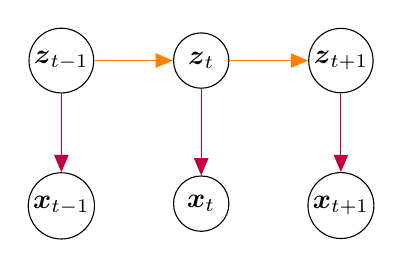
\begin{tikzpicture}
    \node[latent] (zm) {$\bs{z}_{t-1}$};
    \node[latent,right=of zm] (z) {$\bs{z}_t$};
    \node[latent,right=of z] (zp) {$\bs{z}_{t+1}$};
    \node[latent,below=of zm] (xm) {$\bs{x}_{t-1}$};
    \node[latent,below=of z,yshift=-1mm] (x) {$\bs{x}_t$};
    \node[latent,below=of zp] (xp) {$\bs{x}_{t+1}$};
    \draw[->,purple] (zm)--(xm);
    \draw[->,purple] (z)--(x);
    \draw[->,purple] (zp)--(xp);
    \draw[->,orange] (zm)--(z);
    \draw[->,orange] (z)--(zp);
    \end{tikzpicture}
  \end{figure}}%
\end{frame}

%%%%%%%%%%%%%%%%%%%%%%%%%%%%%%%%%%%%%%%%%%%%%%%%%%%%%%%%%%%%%%
\begin{frame}{How does $\mathcal{Q}$ decompose? (II)}
If we develop $\mathcal{Q}$:
  \begin{align*}
   \mathcal{Q} &= \mathbb{E}_{p(\bs{z}_{1:T}|\bs{x}_{1:T};\bar{\bs{\Theta}})} \left\{ \sum_{t=1}^T \log p(\bs{x}_t|\bs{z}_t;\bs{\Theta}) + \sum_{t=2}^T p(\bs{z}_t|\bs{z}_{t-1};\bs{\Theta}) + \log p(\bs{z}_1;\bs{\Theta}) \right\} \\
   &= \sum_{t=1}^T \mathbb{E}_{p(\bs{z}_{t}|\bs{x}_{1:T};\bar{\bs{\Theta}})} \{\log p(\bs{x}_t|\bs{z}_t;\bs{\Theta})\}\\ &+ \sum_{t=2}^T\mathbb{E}_{p(\bs{z}_{t-1},\bs{z}_t|\bs{x}_{1:T};\bar{\bs{\Theta}})}\{ \log p(\bs{z}_t|\bs{z}_{t-1};\bs{\Theta})\} + \mathbb{E}_{p(\bs{z}_{1}|\bs{x}_{1:T};\bar{\bs{\Theta}})}\{\log p(\bs{z}_1;\bs{\Theta}) \}.
  \end{align*}

 In order to compute $\mathcal{Q}$, we need to first compute:
 \begin{equation*}
  p(\bs{z}_t|\bs{x}_{1:T};\bar{\bs{\Theta}}) \quad\text{and}\quad p(\bs{z}_{t-1},\bs{z}_t|\bs{x}_{1:T};\bar{\bs{\Theta}}), \quad \forall t.
 \end{equation*}
\end{frame}

%%%%%%%%%%%%%%%%%%%%%%%%%%%%%%%%%%%%%%%%%%%%%%%%%%%%%%%%%%%%%%
\begin{frame}{Forward-backward -- motivation}
If we start from scratch, we write:
{\small\begin{align*}
 p(\bs{z}_{t}|\bs{x}_{1:T}) &= \int\ldots\int p(\bs{z}_{1:T}|\bs{x}_{1:T}) \textrm{d}\bs{z}_{1:t-1}\textrm{d}\bs{z}_{t+1:T} \\
 &= \frac{1}{p(\bs{x}_{1:T})}\int\ldots\int p(\bs{x}_{1:T},\bs{z}_{1:T}) \textrm{d}\bs{z}_{1:t-1}\textrm{d}\bs{z}_{t+1:T} \\
 &= \frac{1}{p(\bs{x}_{1:T})}\int\ldots\int \prod_{\tau=1}^{T} p(\bs{x}_{\tau}|\bs{z}_{\tau}) \prod_{\tau=2}^{T} p(\bs{z}_{\tau}|\bs{z}_{\tau-1})p(\bs{z}_1) \textrm{d}\bs{z}_{1:t-1}\textrm{d}\bs{z}_{t+1:T}
%  &= \frac{1}{p(\bs{x}_{1:T})}\int\ldots\int \prod_{\tau=1}^{t} p(\bs{x}_{\tau}|\bs{z}_{\tau}) \prod_{\tau=2}^{t} p(\bs{z}_{\tau}|\bs{z}_{\tau-1})p(\bs{z}_1) \textrm{d}\bs{z}_{1:t-1}  \\
%  & \qquad \times\int\ldots\int \prod_{\tau=t+1}^{T} p(\bs{x}_{\tau}|\bs{z}_{\tau}) \prod_{\tau=t+1}^{T} p(\bs{z}_{\tau}|\bs{z}_{\tau-1}) \textrm{d}\bs{z}_{t+1:T}
\end{align*}}

This requires $T-1$ integrals for every $\bs{z}_t$, so $T(T-1)$ integrals.\vspace{3mm}

 We need a \textbf{smarter strategy}!

\end{frame}

\begin{frame}{Forward-backward -- introduction}
 As in the case of HMM, we will use the \textbf{forward-backward} algorithm.\vspace{3mm}
 
 \textbf{Main idea}: decompose as a product of a forward and backward \textit{distributions} that can be computed recursively and re-used at every $t$:
 \begin{align*}
  p(\bs{z}_t|\bs{x}_{1:T}) &\stackrel{(\bs{z}_t)}{\propto} p(\bs{z}_t,\bs{x}_{1:T}) = p(\bs{z}_t,\bs{x}_{1:t}) p(\bs{x}_{t+1:T}|\bs{z}_t)
 \end{align*}
 
\exercise{d-separation-lds}{Prove that the past dependencies drop from the backward term, or equivalently that $\bs{x}_{1:t}$ and $\bs{x}_{t+1:T}$ are D-separated by $\bs{z}_t$.}\vspace{3mm}

 We refer to $p(\bs{z}_t,\bs{x}_{1:t})$ and $p(\bs{x}_{t+1:T}|\bs{z}_t)$ as the forward and backward \textit{distributions}, but this is a language abuse.
 \end{frame}


%%%%%%%%%%%%%%%%%%%%%%%%%%%%%%%%%%%%%%%%%%%%%%%%%%%%%%%%%%%%%%
\begin{frame}{Forward-backward -- general recursions}
We recall $p(\bs{z}_t|\bs{x}_{1:T}) \stackrel{(\bs{z}_{1:T})}{\propto} {\color{mygreen}p(\bs{z}_t,\bs{x}_{1:t})} {\color{myred}p(\bs{x}_{t+1:T}|\bs{z}_t)}$, but also:
{\small\begin{align*}
 p(\bs{z}_{t}|\bs{x}_{1:T}) &= \frac{1}{p(\bs{x}_{1:T})}{\color{mygreen}\int\ldots\int \prod_{\tau=1}^{t} p(\bs{x}_{\tau}|\bs{z}_{\tau}) \prod_{\tau=2}^{t} p(\bs{z}_{\tau}|\bs{z}_{\tau-1})p(\bs{z}_1) \textrm{d}\bs{z}_{1:t-1}}  \\
 & \qquad \times {\color{myred}\int\ldots\int \prod_{\tau=t+1}^{T} p(\bs{x}_{\tau}|\bs{z}_{\tau}) \prod_{\tau=t+1}^{T} p(\bs{z}_{\tau}|\bs{z}_{\tau-1}) \textrm{d}\bs{z}_{t+1:T}}
\end{align*}}
\pause

\exercise{foward-backward-general}{Prove the general forward-backward recursions:
 \begin{align*}
   {\color{mygreen}p(\bs{z}_t,\bs{x}_{1:t})} &= p(\bs{x}_t|\bs{z}_t) \int p(\bs{z}_t|\bs{z}_{t-1}) {\color{mygreen}p(\bs{z}_{t-1},\bs{x}_{1:t-1})} \textrm{d}\bs{z}_{t-1},
 \end{align*}
  \begin{equation*}
  {\color{myred}p(\bs{x}_{t+1:T}|\bs{z}_t)} = \int p(\bs{x}_{t+1}|\bs{z}_{t+1}) p(\bs{z}_{t+1}|\bs{z}_{t}) {\color{myred}p(\bs{x}_{t+2:T}|\bs{z}_{t+1})} \textrm{d}\bs{z}_{t+1}.
 \end{equation*}
}
\end{frame}




%%%%%%%%%%%%%%%%%%%%%%%%%%%%%%%%%%%%%%%%%%%%%%%%%%%%%%%%%%%%%%
\begin{frame}{Forward-backward -- back to efficiency}
 \textbf{Forward}$\quad$ Start with $p(\bs{z}_1|\bs{x}_1)$ and compute: {\small
 \[ {\color{mygreen}p(\bs{z}_t,\bs{x}_{1:t})} = p(\bs{x}_t|\bs{z}_t) \int p(\bs{z}_t|\bs{z}_{t-1}) {\color{mygreen}p(\bs{z}_{t-1},\bs{x}_{1:t-1})} \textrm{d}\bs{z}_{t-1}, \quad\forall t. \]}
 
 \textbf{Backward}$\quad$ Start with $p(\bs{x}_T|\bs{z}_{T-1})$ and compute:
 {\small
  \begin{equation*}
  {\color{myred}p(\bs{x}_{t+1:T}|\bs{z}_t)} = \int p(\bs{x}_{t+1}|\bs{z}_{t+1}) p(\bs{z}_{t+1}|\bs{z}_{t}) {\color{myred}p(\bs{x}_{t+2:T}|\bs{z}_{t+1})} \textrm{d}\bs{z}_{t+1}, \forall t.
 \end{equation*}
 }
 
 \textbf{Posterior}$\quad$ Compute $p(\bs{z}_t|\bs{x}_{1:T})\propto {\color{mygreen}p(\bs{z}_t,\bs{x}_{1:t})}{\color{myred}p(\bs{x}_{t+1:T}|\bs{z}_t)}$, $\forall t$.\vspace{6mm}
 
 This is the exact same formulation as for HMM (we did not use the distributions of $\bs{z}_t$ and $\bs{x}_t$), so this is general. With this strategy, we need $2(T-1)$ integrals, instead of $T(T-1)$.
\end{frame}

%%%%%%%%%%%%%%%%%%%%%%%%%%%%%%%%%%%%%%%%%%%%%%%%%%%%%%%%%%%%%%
\begin{frame}{Back to LDS}
  Out aim is to compute $p(\bs{z}_t|\bs{x}_{1:T})\propto {\color{mygreen}p(\bs{z}_t,\bs{x}_{1:t})}{\color{myred}p(\bs{x}_{t+1:T}|\bs{z}_t)}$, $\forall t$.\vspace{5mm}

  We name ${\color{mygreen}\alpha_t(\bs{z}_t)=p(\bs{z}_t,\bs{x}_{1:t})}$ and ${\color{myred}\beta_t(\bs{z}_t)=p(\bs{x}_{t+1:T}|\bs{z}_t)}$ the forward and backward \textbf{distributions} (recall this language abuse).\vspace{5mm}
  
  We will see that they are all Gaussian distributions.\vspace{5mm}
  
  We will detail the forward recursion (backward for homework) and the initialisation of both recursions. \textcolor{myblue}{Blue will denote the parameters of the model}, \textcolor{mygreen}{green will denote the forward} and \textcolor{myred}{red the backward}.
\end{frame}

%%%%%%%%%%%%%%%%%%%%%%%%%%%%%%%%%%%%%%%%%%%%%%%%%%%%%%%%%%%%%%
\begin{frame}{The forward distribution}
\exercise{forward-lds}{Let us assume: $\paint{mygreen}{\alpha_{t-1}}(\bs{z}_{t-1}) = {\cal N}(\bs{z}_{t-1};\paint{mygreen}{\boldsymbol{\mu}_{t-1}},\paint{mygreen}{\bs{V}_{t-1}})$, prove that the recursion leads to $\paint{mygreen}{\alpha_t}(\bs{z}_t) = \MN(\bs{z}_t; \paint{mygreen}{\bs{\mu}_t}, \paint{mygreen}{\bs{V}_t})$, with:
 \begin{equation*}
 \left\{\begin{array}{l}
 \paint{mygreen}{\bs{V}_t} = \Big(\paint{myblue}{\bs{C}}^\top\paint{myblue}{\bs{\Sigma}}^{-1}\paint{myblue}{\bs{C}} + (\paint{myblue}{\bs{\Gamma}}+\paint{myblue}{\bs{A}}\paint{mygreen}{\bs{V}_{t-1}}\paint{myblue}{\bs{A}}^\top)^{-1}\Big)^{-1},
 \\ \paint{mygreen}{\boldsymbol{\mu}_t}=\paint{mygreen}{\bs{V}_t}\Big( (\paint{myblue}{\bs{\Gamma}}+\paint{myblue}{\bs{A}}\paint{mygreen}{\bs{V}_{t-1}}\paint{myblue}{\bs{A}}^\top)^{-1}\paint{myblue}{\bs{A}}\paint{mygreen}{\boldsymbol{\mu}_{t-1}} + \paint{myblue}{\bs{C}}\paint{myblue}{\bs{\Sigma}}^{-1} \bs{x}_t\Big).
 \end{array}\right.
\end{equation*}
}
\vspace{3mm}
``Intuitively''...
\begin{equation*}
 \paint{mygreen}{\alpha_t}(\bs{z}_t) = \underbrace{p(\bs{x}_t|\bs{z}_t)}_{\MN(\bs{x}_t;\paint{myblue}{\bs{C}}\bs{z}_{t},\paint{myblue}{\bs{\Sigma}})}\int \underbrace{p(\bs{z}_t|\bs{z}_{t-1})}_{\MN(\bs{z}_t;\paint{myblue}{\bs{A}}\bs{z}_{t-1},\paint{myblue}{\bs{\Gamma}})}\underbrace{\paint{mygreen}{\alpha_{t-1}}(\bs{z}_{t-1})}_{{\cal N}(\bs{z}_{t-1};\paint{mygreen}{\boldsymbol{\mu}_{t-1}},\paint{mygreen}{\bs{V}_{t-1}})}\textrm{d}\bs{z}_{t-1}.
\end{equation*}

\end{frame}
% 
% \begin{frame}
% We recall that $p(\bs{z}_t|\bs{z}_{t-1}) = \MN(\bs{z}_t;\paint{myblue}{\bs{A}}\bs{z}_{t-1},\paint{myblue}{\bs{\Gamma}})$, and
%  \begin{equation*}
%    \paint{mygreen}{\alpha_t}(\bs{z}_t) = p(\bs{x}_t|\bs{z}_t)\int p(\bs{z}_t|\bs{z}_{t-1})\paint{mygreen}{\alpha_{t-1}}(\bs{z}_{t-1})\textrm{d}\bs{z}_{t-1}.
%  \end{equation*}\pause
%  Let us assume that $\alpha_{t-1}(\bs{z}_{t-1}) = \MN(\bs{z}_{t-1};\paint{mygreen}{\bs{\mu}_{t-1}},\paint{mygreen}{\bs{V}_{t-1}})$, then:
%  \begin{equation*}
%   \int p(\bs{z}_t|\bs{z}_{t-1})\paint{mygreen}{\alpha_{t-1}}(\bs{z}_{t-1})\textrm{d}\bs{z}_{t-1} = \MN(\bs{z}_t;\paint{myblue}{\bs{A}}\paint{mygreen}{\bs{\mu}_{t-1}},\paint{myblue}{\bs{\Gamma}}+\paint{myblue}{\bs{A}}\paint{mygreen}{\bs{V}_{t-1}}\paint{myblue}{\bs{A}}^\top).
%  \end{equation*}\pause
%  We also recall that $p(\bs{x}_t|\bs{z}_t) = \MN(\bs{x}_t;\paint{myblue}{\bs{C}}\bs{z}_t,\paint{myblue}{\bs{\Sigma}})$, then we obtain {\small(\textbf{homework})}:
%  \begin{equation*}
%   \alpha_t(\bs{z}_t) = \MN(\bs{z}_t; \paint{mygreen}{\bs{\mu}_t}, \paint{mygreen}{\bs{V}_t}),
%  \end{equation*}
%  \small
%  \begin{equation*}\text{with}\quad 
%  \left\{\begin{array}{l}
%  \paint{mygreen}{\bs{V}_t} = \Big(\paint{myblue}{\bs{C}}^\top\paint{myblue}{\bs{\Sigma}}^{-1}\paint{myblue}{\bs{C}} + (\paint{myblue}{\bs{\Gamma}}+\paint{myblue}{\bs{A}}\paint{mygreen}{\bs{V}_{t-1}}\paint{myblue}{\bs{A}}^\top)^{-1}\Big)^{-1},
%  \\ \paint{mygreen}{\boldsymbol{\mu}_t}=\paint{mygreen}{\bs{V}_t}\Big( (\paint{myblue}{\bs{\Gamma}}+\paint{myblue}{\bs{A}}\paint{mygreen}{\bs{V}_{t-1}}\paint{myblue}{\bs{A}}^\top)^{-1}\paint{myblue}{\bs{A}}\paint{mygreen}{\boldsymbol{\mu}_{t-1}} + \paint{myblue}{\bs{C}}\paint{myblue}{\bs{\Sigma}}^{-1} \bs{x}_t\Big).
%  \end{array}\right.
% \end{equation*}
% \end{frame}

%%%%%%%%%%%%%%%%%%%%%%%%%%%%%%%%%%%%%%%%%%%%%%%%%%%%%%%%%%%%%%
\begin{frame}{The backward and posterior distributions}
\exercise{backward-lds}{Prove that if $\paint{myred}{\beta_{t+1}}(\bs{z}_{t+1})={\cal N}(\bs{z}_{t+1};\paint{myred}{\boldsymbol{\nu}_{t+1}},\paint{myred}{\bs{W}_{t+1}})$, then $\paint{myred}{\beta_t}(\bs{z}_t) = {\cal N}(\bs{z}_t;\paint{myred}{\boldsymbol{\nu}_t},\paint{myred}{\bs{W}_t})$ with:
{\small\begin{equation*}
\left\{\begin{array}{l}  \paint{myred}{\bs{W}_t^{-1}} = \paint{myblue}{\bs{A}^\top}(\paint{myblue}{\bs{\Gamma}} + (\paint{myred}{\bs{W}_{t+1}^{-1}} + \paint{myblue}{\bs{C}^\top\bs{\Sigma}^{-1}\bs{C}})^{-1})^{-1}\paint{myblue}{\bs{A}}\\
\paint{myred}{\boldsymbol{\nu}_t} = \paint{myred}{\bs{W}_t} \paint{myblue}{\bs{A}^\top\bs{\Gamma}^{-1}}(\paint{myblue}{\bs{C}^\top\bs{\Sigma}^{-1}\bs{C}} + \paint{myred}{\bs{W}_{t+1}^{-1}} + \paint{myblue}{\bs{\Gamma}^{-1}})^{-1} ( \paint{myblue}{\bs{C}^\top\bs{\Sigma}^{-1}}\bs{x}_{t+1} + \paint{myred}{\bs{W}_{t+1}^{-1}\boldsymbol{\nu}_{t+1}})
\end{array}\right.
\end{equation*}}
}\vspace{2mm}
%   We can use a similar strategy for the backward distribution. If we assume that $\paint{myred}{\beta_{t+1}}(\bs{z}_{t+1}) = \MN(\bs{z}_{t+1},\paint{myred}{\bs{\nu}_{t+1}},\paint{myred}{\bs{W}_{t+1}})$, then {(\textbf{homework})}:
%   \begin{equation*}
%     \paint{myred}{\beta_t}(\bs{z}_t) = \MN(\bs{z}_t;\paint{myred}{\bs{\nu}_t},\paint{myred}{\bs{W}_t})
% \end{equation*}
% with $\paint{myred}{\bs{W}_t}^{-1} = \paint{myblue}{\bs{A}}^\top(\paint{myblue}{\bs{\Gamma}} + (\paint{myred}{\bs{W}_{t+1}}^{-1} + \paint{myblue}{\bs{C}}^\top\paint{myblue}{\bs{\Sigma}}^{-1}\paint{myblue}{\bs{C}})^{-1})^{-1}\paint{myblue}{\bs{A}}$ and:
% {\small \begin{equation*}
% \paint{myred}{\boldsymbol{\nu}_t} = \paint{myred}{\bs{W}_t} \paint{myblue}{\bs{A}}^\top\paint{myblue}{\bs{\Gamma}}^{-1}(\paint{myblue}{\bs{C}}^\top\paint{myblue}{\bs{\Sigma}}^{-1}\paint{myblue}{\bs{C}} + \paint{myred}{\bs{W}_{t+1}}^{-1}+\paint{myblue}{\bs{\Gamma}}^{-1})^{-1} (\paint{myblue}{\bs{C}}^\top\paint{myblue}{\bs{\Sigma}}^{-1}\bs{x}_{t+1} + \paint{myred}{\bs{W}_{t+1}}^{-1}\paint{myred}{\boldsymbol{\nu}_{t+1}}).
% \end{equation*}}

Now we can deduce that:
\begin{equation*}
 p(\bs{z}_t|\bs{x}_{1:T}) \stackrel{(\bs{z}_t)}{\propto} \paint{mygreen}{\alpha_t}(\bs{z}_t)\paint{myred}{\beta_t}(\bs{z}_t) \stackrel{(\bs{z}_t)}{\propto} \MN(\bs{z}_t;\bs{m}_t,\bs{\Lambda}_{t})
\end{equation*}
with
\begin{equation*}
 \bs{\Lambda}_{t} = (\paint{mygreen}{\bs{V}_t}^{-1}+\paint{myred}{\bs{W}_t}^{-1})^{-1} \qquad \bs{m}_t = \bs{\Lambda}_{t}(\paint{mygreen}{\bs{V}_t}^{-1}\paint{mygreen}{\boldsymbol{\mu}_t} + \paint{myred}{\bs{W}_t}^{-1}\paint{myred}{\boldsymbol{\nu}_t})
\end{equation*}\pause
But how to initialise the recursions?
\end{frame}

% %%%%%%%%%%%%%%%%%%%%%%%%%%%%%%%%%%%%%%%%%%%%%%%%%%%%%%%%%%%%%%
% \begin{frame}{Let's take a breath}
%  \begin{center}\Large ANY QUESTIONS?\end{center}
% \end{frame}

%%%%%%%%%%%%%%%%%%%%%%%%%%%%%%%%%%%%%%%%%%%%%%%%%%%%%%%%%%%%%%
\begin{frame}{Forward-backward initialisation}
%  The forward and the backward recursions need to be initialised.\vspace{3mm}
 
 \textbf{Forward}:
 \begin{align*}
  \paint{mygreen}{\alpha_1}(\bs{z}_1) &= p(\bs{x}_1|\bs{z}_1)p(\bs{z}_1) = \MN(\bs{x}_1;\paint{myblue}{\bs{C}}\bs{z}_1,\paint{myblue}{\bs{\Sigma}})\MN(\bs{z}_1;\paint{myblue}{\bs{d}},\paint{myblue}{\bs{\Omega}})\\
  &={\cal N}(\bs{z}_1;\paint{mygreen}{\boldsymbol{\mu}_1},\paint{mygreen}{\bs{V}_1}) \text{ with } \left\{\begin{array}{l} \paint{mygreen}{\bs{V}_1} = (\paint{myblue}{\bs{\Omega}^{-1}} + \paint{myblue}{\bs{C}}\paint{myblue}{\bs{\Sigma}^{-1}}\paint{myblue}{\bs{C}^\top})^{-1}, \\ \paint{mygreen}{\boldsymbol{\mu}_1} = \paint{mygreen}{\bs{V}_1}(\paint{myblue}{\bs{\Omega}^{-1}}\paint{myblue}{\bs{d}} + \paint{myblue}{\bs{C}^\top}\paint{myblue}{\bs{\Sigma}^{-1}}\bs{x}_1)\end{array}\right.
 \end{align*}\pause\vspace{3mm}
 
 \textbf{Backward}: Notice that $p(\bs{z}_T|\bs{x}_{1:T})=\alpha_T(\bs{z}_T)\beta_T(\bs{z}_T)$, but $\alpha_T(\bs{z}_T)\propto p(\bs{z}_T|\bs{x}_{1:T})$ by definition, so $\beta_T\propto 1$.\vspace{3mm}\\

 As in the HMM case, $\paint{myred}{\beta_T}$ should be non-informative or ``uniform.''
 \small\begin{equation*}
  \paint{myred}{\bs{W}_T^{-1}}\rightarrow 0 \Rightarrow \left\{\begin{array}{l}
  \paint{myred}{\bs{W}_{T-1}^{-1}} = \paint{myblue}{\bs{A}^\top}(\paint{myblue}{\bs{\Gamma}} + (\paint{myblue}{\bs{C}^\top}\paint{myblue}{\bs{\Sigma}^{-1}}\paint{myblue}{\bs{C}})^{-1})^{-1}\paint{myblue}{\bs{A}} \\
  \paint{myred}{\boldsymbol{\nu}_{T-1}} = \paint{myred}{\bs{W}_{T-1}} \paint{myblue}{\bs{A}^\top}\paint{myblue}{\bs{\Gamma}^{-1}}(\paint{myblue}{\bs{C}^\top}\paint{myblue}{\bs{\Sigma}^{-1}}\paint{myblue}{\bs{C}} + \paint{myblue}{\bs{\Gamma}^{-1}})^{-1} (\paint{myblue}{\bs{C}^\top}\paint{myblue}{\bs{\Sigma}^{-1}}\bs{x}_{t+1}).
  \end{array}\right.
 \end{equation*}
 This is equivalent to start from $\paint{myred}{\beta_{T-1}}(\bs{z}_{T-1}) = \int p(\bs{x}_T,\bs{z}_T|\bs{z}_{T-1})\textrm{d}\bs{z}_{T-1}$.
\end{frame}


%%%%%%%%%%%%%%%%%%%%%%%%%%%%%%%%%%%%%%%%%%%%%%%%%%%%%%%%%%%%%%
\begin{frame}{Recap and notations}
  We can now compute $p(\bs{z}_t|\bs{x}_{1:T};\bar{\bs{\Theta}})$ (previous formulae):
  \begin{itemize}
   \item Initialise and compute the parameters of the forward distribution.
   \item Initialise and compute the parameters of the backward distribution.
   \item Compute the parameters of the posterior.
  \end{itemize}\vspace{3mm}
  
  In the previous equations we droped the bar from $\bar{\bs{\Theta}}$ for simplicity. For the E-step ALWAYS use the parameters of the previous iteration!\\
  (So all equations above should use $\bar{\bs{A}}$, $\bar{\bs{\Gamma}}$, $\bar{\bs{C}}$, $\bar{\bs{\Sigma}}$, $\bar{\bs{d}}$ and $\bar{\bs{\Omega}}$)\vspace{3mm}

  To finish the E-step, we need to compute the joint distribution $p(\bs{z}_t,\bs{z}_{t+1}|\bs{x}_{1:T})$.
%   
%   \small
%  \begin{equation*}
%  p(\bs{z}_t|\bs{x}_{1:T}) = \MN(\bs{z}_t;\bs{m}_t,\bs{\Lambda}_{t}) \text{ with } \left\{ \begin{array}{l} \bs{\Lambda}_{t} = (\paint{mygreen}{\bs{V}_t}^{-1}+\paint{myred}{\bs{W}_t}^{-1})^{-1} \\ \bs{m}_t = \bs{\Lambda}_{t}(\paint{mygreen}{\bs{V}_t}^{-1}\paint{mygreen}{\boldsymbol{\mu}_t} + \paint{myred}{\bs{W}_t}^{-1}\paint{myred}{\boldsymbol{\nu}_t}) \end{array}\right.
% \end{equation*}\vspace{-3mm}
% \begin{columns}
%  \begin{column}{0.3\textwidth}
%   where $\paint{mygreen}{\boldsymbol{\mu}_t}$ and $\paint{mygreen}{\bs{V}_t}$ are computed with forward recursions:
%  \end{column}\hspace{-5mm}
%  \begin{column}{0.75\textwidth}
%  \vspace{-2mm}
%  \begin{equation*}
%  \left\{\begin{array}{l}
%  \paint{mygreen}{\bs{V}_t} = \Big(\paint{myblue}{\bs{C}}^\top\paint{myblue}{\bs{\Sigma}}^{-1}\paint{myblue}{\bs{C}} + (\paint{myblue}{\bs{\Gamma}}+\paint{myblue}{\bs{A}}\paint{mygreen}{\bs{V}_{t-1}}\paint{myblue}{\bs{A}}^\top)^{-1}\Big)^{-1},
%  \\ \paint{mygreen}{\boldsymbol{\mu}_t}=\paint{mygreen}{\bs{V}_t}\Big( (\paint{myblue}{\bs{\Gamma}}+\paint{myblue}{\bs{A}}\paint{mygreen}{\bs{V}_{t-1}}\paint{myblue}{\bs{A}}^\top)^{-1}\paint{myblue}{\bs{A}}\paint{mygreen}{\boldsymbol{\mu}_{t-1}} + \paint{myblue}{\bs{C}}\paint{myblue}{\bs{\Sigma}}^{-1} \bs{x}_t\Big), 
%  \end{array}\right.
% \end{equation*}
%  \end{column}
% \end{columns}\vspace{1mm}
% and $\paint{myred}{\boldsymbol{\nu}_t}$ and $\paint{myred}{\bs{W}_t}$ with backward recursions. The joint distribution $p(\bs{z}_t,\bs{z}_{t+1}|\bs{x}_{1:T})$ uses the \textcolor{green}{forward}, \textcolor{red}{backward} and \textcolor{blue}{model parameters} \textbf{of the previous iteration} $\bar{\bs{\Theta}}$.\vspace{3mm}
% 
% But presenting the previous equations with $\bs{A}^o$, $\bs{\Gamma}^o$, $\bs{C}^o$, $\bs{\Sigma}^o$, $\bs{d}$ and $\bs{\Omega}$, is very tedious and confusing. When computing the E-step ALWAYS use the model parameters of the previous iteration!
\end{frame}


%%%%%%%%%%%%%%%%%%%%%%%%%%%%%%%%%%%%%%%%%%%%%%%%%%%%%%%%%%%%%%
\begin{frame}{The joint posterior}
 In addition to $p(\bs{z}_t|\bs{x}_{1:T})$ we also need $p(\bs{z}_t,\bs{z}_{t+1}|\bs{x}_{1:T})$:
 \footnotesize
 \begin{align*}
 &p(\bs{z}_t,\bs{z}_{t+1}|\bs{x}_{1:T}) = \int\ldots\int p(\bs{z}_{1:T}|\bs{x}_{1:T})\textrm{d}\bs{z}_{1:t-1}\textrm{d}\bs{z}_{t+2:T} \\
 &\stackrel{(\bs{z}_t,\bs{z}_{t+1})}{\propto} \paint{mygreen}{\alpha_t}(\bs{z}_t)p(\bs{x}_{t+1}|\bs{z}_{t+1})p(\bs{z}_{t+1}|\bs{z}_t)\paint{myred}{\beta_{t+1}}(\bs{z}_{t+1})\\
 &\stackrel{(\bs{z}_t,\bs{z}_{t+1})}{\propto} {\cal N}(\bs{z}_t;\paint{mygreen}{\boldsymbol{\mu}_t,\bs{V}_t}) {\cal N}(\bs{x}_{t+1};\paint{myblue}{\bs{C}}\bs{z}_{t+1},\paint{myblue}{\bs{\Sigma}}) {\cal N}(\bs{z}_{t+1};\paint{myblue}{\bs{A}}\bs{z}_t,\paint{myblue}{\bs{\Gamma}}) {\cal N}(\bs{z}_{t+1};\paint{myred}{\boldsymbol{\nu}_{t+1}},\paint{myred}{\bs{W}_{t+1}})
\end{align*}
\normalsize
\only<1>{What kind of distribution is this going to be?}\vspace{3mm}
\pause

% So this is going to be a Gaussian distribution on $[\bs{z}_t,\bs{z}_{t+1}]$!
Yes! $p(\bs{z}_t,\bs{z}_{t+1}|\bs{x}_{1:T}) = {\cal N}([\bs{z}_{t};\bs{z}_{t+1}]; \bs{\xi}_t,\bs{\Xi}_t)$ with:
{ \footnotesize
\begin{equation*}
 \bs{\Xi}_t = \myarray{cc}{\paint{mygreen}{\bs{V}_t}^{-1}+\paint{myblue}{\bs{A}}^\top\paint{myblue}{\bs{\Gamma}}^{-1}\paint{myblue}{\bs{A}} & -\paint{myblue}{\bs{A}}^\top\paint{myblue}{\bs{\Gamma}}^{-1}\\-\paint{myblue}{\bs{\Gamma}}^{-1}\paint{myblue}{\bs{A}} & \paint{myred}{\bs{W}_{t+1}}^{-1} + \paint{myblue}{\bs{\Gamma}}^{-1} + \paint{myblue}{\bs{C}}^\top\paint{myblue}{\bs{\Sigma}}^{-1}\paint{myblue}{\bs{C}}}^{-1}
\end{equation*}}
and:
{ \footnotesize\begin{equation*}
 \bs{\xi}_t = \bs{\Xi}_t\myarray{c}{\paint{mygreen}{\bs{V}_t}^{-1}\paint{mygreen}{\boldsymbol{\mu}_t}\\\paint{myblue}{\bs{C}}^\top\paint{myblue}{\bs{\Sigma}}^{-1}\bs{x}_{t+1} + \paint{myred}{\bs{W}_{t+1}}^{-1}\paint{myred}{\boldsymbol{\nu}_{t+1}}}.
 \end{equation*}}
\end{frame}

% %%%%%%%%%%%%%%%%%%%%%%%%%%%%%%%%%%%%%%%%%%%%%%%%%%%%%%%%%%%%%%
% \begin{frame}{The joint posterior (II)}
% \textbf{Homework}: If we write $p(\bs{z}_t,\bs{z}_{t+1}|\bs{x}_{1:T}) = {\cal N}([\bs{z}_{t};\bs{z}_{t+1}]; \bs{\xi}_t,\bs{\Xi}_t)$
% prove:
% \begin{equation*}
%  \bs{\Xi}_t = \myarray{cc}{\paint{mygreen}{\bs{V}_t}^{-1}+\paint{myblue}{\bs{A}}^\top\paint{myblue}{\bs{\Gamma}}^{-1}\paint{myblue}{\bs{A}} & -\paint{myblue}{\bs{A}}^\top\paint{myblue}{\bs{\Gamma}}^{-1}\\-\paint{myblue}{\bs{\Gamma}}^{-1}\paint{myblue}{\bs{A}} & \paint{myred}{\bs{W}_{t+1}}^{-1} + \paint{myblue}{\bs{\Gamma}}^{-1} + \paint{myblue}{\bs{C}}^\top\paint{myblue}{\bs{\Sigma}}^{-1}\paint{myblue}{\bs{C}}}^{-1}
% \end{equation*}
% and:
% \begin{equation*}
%  \bs{\xi}_t = \bs{\Xi}_t\myarray{c}{\paint{mygreen}{\bs{V}_t}^{-1}\paint{mygreen}{\boldsymbol{\mu}_t}\\\paint{myblue}{\bs{C}}^\top\paint{myblue}{\bs{\Sigma}}^{-1}\bs{x}_{t+1} + \paint{myred}{\bs{W}_{t+1}}^{-1}\paint{myred}{\boldsymbol{\nu}_{t+1}}}. \end{equation*}
% If we now define the parts of the mean vector and covariance matrix corresponding to time $t$ and to time $t+1$ as ``$-$'' and ``$+$'' respectively:
% \begin{equation*}
%  \bs{\xi}_t =: \myarray{c}{\bs{\xi}_{t-}\\\bs{\xi}_{t+}} \qquad \bs{\Xi}_t =: \myarray{cc}{ \bs{\Xi}_{t--} & \bs{\Xi}_{t-+} \\ \bs{\Xi}_{t+-} & \bs{\Xi}_{t++}},
% \end{equation*}
% give the expressions for $\bs{\xi}_{t-}$, $\bs{\xi}_{t+}$, $\bs{\Xi}_{t--}$ $\bs{\Xi}_{t-+}$, $\bs{\Xi}_{t+-}$ and $\bs{\Xi}_{t++}$.
%  \end{frame}

% %%%%%%%%%%%%%%%%%%%%%%%%%%%%%%%%%%%%%%%%%%%%%%%%%%%%%%%%%%%%%%
% \begin{frame}{Recap}
%  We need $p(\bs{z}_t|\bs{x}_{1:T};\bar{\bs{\Theta}})$ and $p(\bs{z}_t,\bs{z}_{t+1}|\bs{x}_{1:T};\bar{\bs{\Theta}})$:\small
%  \begin{equation*}
%  p(\bs{z}_t|\bs{x}_{1:T}) = \MN(\bs{z}_t;\bs{m}_t,\bs{\Lambda}_{t}) \text{ with } \left\{ \begin{array}{l} \bs{\Lambda}_{t} = (\paint{mygreen}{\bs{V}_t}^{-1}+\paint{myred}{\bs{W}_t}^{-1})^{-1} \\ \bs{m}_t = \bs{\Lambda}_{t}(\paint{mygreen}{\bs{V}_t}^{-1}\paint{mygreen}{\boldsymbol{\mu}_t} + \paint{myred}{\bs{W}_t}^{-1}\paint{myred}{\boldsymbol{\nu}_t}) \end{array}\right.
% \end{equation*}\vspace{-3mm}
% \begin{columns}
%  \begin{column}{0.3\textwidth}
%   where $\paint{mygreen}{\boldsymbol{\mu}_t}$ and $\paint{mygreen}{\bs{V}_t}$ are computed with forward recursions:
%  \end{column}\hspace{-5mm}
%  \begin{column}{0.75\textwidth}
%  \vspace{-2mm}
%  \begin{equation*}
%  \left\{\begin{array}{l}
%  \paint{mygreen}{\bs{V}_t} = \Big(\paint{myblue}{\bs{C}}^\top\paint{myblue}{\bs{\Sigma}}^{-1}\paint{myblue}{\bs{C}} + (\paint{myblue}{\bs{\Gamma}}+\paint{myblue}{\bs{A}}\paint{mygreen}{\bs{V}_{t-1}}\paint{myblue}{\bs{A}}^\top)^{-1}\Big)^{-1},
%  \\ \paint{mygreen}{\boldsymbol{\mu}_t}=\paint{mygreen}{\bs{V}_t}\Big( (\paint{myblue}{\bs{\Gamma}}+\paint{myblue}{\bs{A}}\paint{mygreen}{\bs{V}_{t-1}}\paint{myblue}{\bs{A}}^\top)^{-1}\paint{myblue}{\bs{A}}\paint{mygreen}{\boldsymbol{\mu}_{t-1}} + \paint{myblue}{\bs{C}}\paint{myblue}{\bs{\Sigma}}^{-1} \bs{x}_t\Big), 
%  \end{array}\right.
% \end{equation*}
%  \end{column}
% \end{columns}\vspace{1mm}
% and $\paint{myred}{\boldsymbol{\nu}_t}$ and $\paint{myred}{\bs{W}_t}$ with backward recursions. The joint distribution $p(\bs{z}_t,\bs{z}_{t+1}|\bs{x}_{1:T})$ uses the \textcolor{green}{forward}, \textcolor{red}{backward} and \textcolor{blue}{model parameters} \textbf{of the previous iteration} $\bar{\bs{\Theta}}$.\vspace{3mm}
% 
% But presenting the previous equations with $\bs{A}^o$, $\bs{\Gamma}^o$, $\bs{C}^o$, $\bs{\Sigma}^o$, $\bs{d}$ and $\bs{\Omega}$, is very tedious and confusing. When computing the E-step ALWAYS use the model parameters of the previous iteration!
% \end{frame}

%%%%%%%%%%%%%%%%%%%%%%%%%%%%%%%%%%%%%%%%%%%%%%%%%%%%%%%%%%%%%
\begin{frame}{Tools for computing $\mathcal{Q}$ and the M-step}
 We recall this important result.\vspace{3mm}\\
 \exercise{expectation-log-gaussian}{The following two formulae hold:
\[
 \expectation[\mathcal{N}(\bs{z};\bs{\mu},\bs{\Sigma})]{\bs{A}\bs{z}} = \bs{A}\bs{\mu} \quad\text{and}\quad \expectation[\mathcal{N}(\bs{z};\bs{\mu},\bs{\Sigma})]{\bs{z}^\top\bs{\Lambda}\bs{z}} = \bs{\mu}^\top\bs{\Lambda}\bs{\mu} + \textrm{Tr}(\bs{\Lambda}\bs{\Sigma}).  
\]
}\vspace{3mm}

We recall certain properties:
 {\small
 \begin{equation*}
 (i)\;\textrm{Tr}(\bs{A}\bs{B}\bs{C}) = \textrm{Tr}(\bs{B}\bs{C}\bs{A}) \qquad 
 (ii)\;\frac{\partial }{\partial \bs{A}} \textrm{Tr}(\bs{A}^\top \bs{B}) = \bs{B}
\end{equation*}
\begin{equation*}
 (iii)\; \frac{\partial }{\partial \bs{A}} \textrm{Tr}(\bs{A} \bs{B} \bs{A}^{\top} \bs{C}) = \bs{C}\bs{A}\bs{B}+\bs{C}^\top\bs{A}\bs{B}^\top \qquad 
 (iv)\; \frac{\partial }{\partial \bs{A}} \log|\bs{A}| = (\bs{A}^{-1})^\top
\end{equation*}}
\end{frame}

%%%%%%%%%%%%%%%%%%%%%%%%%%%%%%%%%%%%%%%%%%%%%%%%%%%%%%%%%%%%%
\begin{frame}{Computing $\mathcal{Q}$ and the M-step}
Let's recall that the posterior distributions:
\begin{equation*}
 p(\bs{z}_t|\bs{x}_{1:T}) = \MN(\bs{z}_t;\bs{m}_t,\bs{\Lambda}_{t})
\end{equation*}
\begin{equation*}
 p(\bs{z}_t,\bs{z}_{t+1}|\bs{x}_{1:T}) = {\cal N}([\bs{z}_{t};\bs{z}_{t+1}]; \bs{\xi}_t,\bs{\Xi}_t)
\end{equation*}
{\small ($\bs{m}_t\in\mathbb{R}^{d_z}$, $\bs{\Lambda}_{t}\in\mathbb{R}^{d_z\times d_z}$ and $\bs{\xi}_t\in\mathbb{R}^{2d_z}$, $\bs{\Xi}_t\in\mathbb{R}^{2d_z\times2d_z}$)}\vspace{3mm}\\

Let us also recall the expresion of the $\mathcal{Q}$ function (derived previously):
  \begin{align*}
   \mathcal{Q} &= \underbrace{\sum_{t=1}^T \mathbb{E}_{p(\bs{z}_{t}|\bs{x}_{1:T};\bar{\bs{\Theta}})} \{\log p(\bs{x}_t|\bs{z}_t;\bs{\Theta})\}}_{\mathcal{Q}_{\bs{C},\bs{\Sigma}}}\\ &+ \underbrace{\sum_{t=2}^T\mathbb{E}_{p(\bs{z}_{t-1},\bs{z}_t|\bs{x}_{1:T};\bar{\bs{\Theta}})}\{ \log p(\bs{z}_t|\bs{z}_{t-1};\bs{\Theta})\}}_{\mathcal{Q}_{\bs{A},\bs{\Gamma}}} + \underbrace{\mathbb{E}_{p(\bs{z}_{1}|\bs{x}_{1:T};\bar{\bs{\Theta}})}\{\log p(\bs{z}_1;\bs{\Theta}) \}}_{\mathcal{Q}_{\bs{d},\bs{\Omega}}}
  \end{align*}
\end{frame}

%%%%%%%%%%%%%%%%%%%%%%%%%%%%%%%%%%%%%%%%%%%%%%%%%%%%%%%%%%%%%
\begin{frame}{M-step: $\bs{C}$ and $\bs{\Sigma}$}
 The expectation of the $t$-th term writes:
 \begin{align*}
  \mathbb{E}_{p(\bs{z}_{t}|\bs{x}_{1:T};\bar{\bs{\Theta}})} & \{\log p(\bs{x}_t|\bs{z}_t;\bs{\Theta})\} \stackrel{(\bs{\Theta})}{=}-\frac{1}{2}\log|\bs{\Sigma}|\\
   & -\frac{1}{2}\textrm{Tr}\left\{\bs{\Sigma}^{-1}\Big( \bs{x}_{t}\bs{x}_{t}^\top - 2\bs{C}\bs{m}_{t}\bs{x}_{t}^\top +\bs{C}(\bs{m}_{t}\bs{m}_{t}^\top + \bs{\Lambda}_{t})\bs{C}^\top  \Big)\right\}
 \end{align*}\pause
 
 Sum over $t$: \only<3->{(\footnotesize $\bs{S}_{xx} = \sum_{t=1}^T \bs{x}_t\bs{x}_t^\top \quad \bs{S}_{zx} = \sum_{t=1}^T \bs{m}\bs{x}^\top \quad \bs{S}_{zz} = \sum_{t=1}^T \bs{m}_t\bs{m}_t^\top + \bs{\Lambda}_{t}$)}
 {\small
  \only<2>{\begin{align*}
  \mathcal{Q}_{\bs{C},\bs{\Sigma}} = -\frac{T}{2}\log|\bs{\Sigma}| -\frac{1}{2}\textrm{Tr}\left\{\bs{\Sigma}^{-1}\sum_{t=1}^T\Big( \bs{x}_{t}\bs{x}_{t}^\top - 2\bs{C}\bs{m}_{t}\bs{x}_{t}^\top +\bs{C}(\bs{m}_{t}\bs{m}_{t}^\top + \bs{\Lambda}_{t})\bs{C}^\top  \Big)\right\}
 \end{align*}}%
  \only<3->{\begin{align*}
  \mathcal{Q}_{\bs{C},\bs{\Sigma}} = -\frac{T}{2}\log|\bs{\Sigma}| -\frac{1}{2}\textrm{Tr}\left\{\bs{\Sigma}^{-1}\Big( \bs{S}_{xx} - 2\bs{C}\bs{S}_{zx} +\bs{C}\bs{S}_{zz}\bs{C}^\top  \Big)\right\}
 \end{align*}}
 }\pause
 
 \begin{equation*}
  \frac{\partial \mathcal{Q}}{\partial \bs{C}}=0 \Rightarrow \bs{C}^* = \bs{S}_{xz}( \bs{S}_{zz})^{-1}
\qquad
 \frac{\partial \mathcal{Q}}{\partial \bs{\Sigma}^{-1}}=0 \Rightarrow \bs{\Sigma}^* = \frac{1}{T}\Big(\bs{S}_{xx} - \bs{S}_{xz}( \bs{S}_{zz})^{-1}\bs{S}_{zx}\Big)
\end{equation*}
\end{frame}

% %%%%%%%%%%%%%%%%%%%%%%%%%%%%%%%%%%%%%%%%%%%%%%%%%%%%%%%%%%%%%
% \begin{frame}{M-step: $\bs{C}$ and $\bs{\Sigma}$ (II)}
%  Let's sum over $t$:
%  {\small
%  \begin{align*}
%   Q&\stackrel{(\bs{C},\bs{\Sigma})}{=} \sum_{t=1}^T \mathbb{E}_{p(\bs{z}_{t}|\bs{x}_{1:T};\bar{\bs{\Theta}})} \{\log p(\bs{x}_t|\bs{z}_t;\bs{\Theta})\} \\
%   &\stackrel{(\bs{C},\bs{\Sigma})}{=} -\frac{T}{2}\log|\bs{\Sigma}| -\frac{1}{2}\sum_{t=1}^T \textrm{Tr}\left\{\bs{\Sigma}^{-1}\Big( \bs{x}_{t}\bs{x}_{t}^\top - 2\bs{C}\bs{m}_{t}\bs{x}_{t}^\top +\bs{C}(\bs{m}_{t}\bs{m}_{t}^\top + \bs{\Lambda}_{t})\bs{C}^\top  \Big)\right\}
%  \end{align*}
%  }\vspace{3mm}
%  
%  We ``take the sum inside the trace'' and define:
%  \begin{equation*}
%   \bs{S}_{xx} = \sum_{t=1}^T \bs{x}_t\bs{x}_t^\top \quad \bs{S}_{zx} = \sum_{t=1}^T \bs{m}\bs{x}^\top \quad \bs{S}_{zz} = \sum_{t=1}^T \bs{m}_t\bs{m}_t^\top + \bs{\Lambda}_{t} 
%  \end{equation*}
% 
% \end{frame}
% 
% %%%%%%%%%%%%%%%%%%%%%%%%%%%%%%%%%%%%%%%%%%%%%%%%%%%%%%%%%%%%%
% \begin{frame}{M-step: $\bs{C}$ and $\bs{\Sigma}$ (III)}
%  With this we can rewrite the part of $Q$ that depends on $\bs{C}$ and $\bs{\Sigma}$ as:
%   {\small
%  \begin{align*}
%   Q\stackrel{(\bs{C},\bs{\Sigma})}{=} -\frac{T}{2}\log|\bs{\Sigma}| -\frac{1}{2} \textrm{Tr}\left\{\bs{\Sigma}^{-1}\Big( \bs{S}_{xx} - 2\bs{C}\bs{S}_{zx} +\bs{C}\bs{S}_{zz}\bs{C}^\top  \Big)\right\}
%  \end{align*}
%  }
%  We recall certain properties:
%  {\small
%  \begin{equation*}
%  (i)\;\textrm{Tr}(\bs{A}\bs{B}\bs{C}) = \textrm{Tr}(\bs{B}\bs{C}\bs{A}) \qquad 
%  (ii)\;\frac{\partial }{\partial \bs{A}} \textrm{Tr}(\bs{A}^\top \bs{B}) = \bs{B}
% \end{equation*}
% \begin{equation*}
%  (iii)\; \frac{\partial }{\partial \bs{A}} \textrm{Tr}(\bs{A} \bs{B} \bs{A}^{\top} \bs{C}) = \bs{C}\bs{A}\bs{B}+\bs{C}^\top\bs{A}\bs{B}^\top \qquad 
%  (iv)\; \frac{\partial }{\partial \bs{A}} \log|\bs{A}| = (\bs{A}^{-1})^\top
% \end{equation*}}\vspace{3mm}
% \only<1>{Prove that (5 min):
% \begin{equation*}
%  \frac{\partial Q}{\partial \bs{C}}=0 \Rightarrow \bs{C}^* = \bs{S}_{xz}( \bs{S}_{zz})^{-1}
% \end{equation*}
% }%
% \only<2>{Prove that (5 min):
% \begin{equation*}
%  \frac{\partial Q}{\partial \bs{\Sigma}^{-1}}=0 \Rightarrow \bs{\Sigma}^* = \frac{1}{T}\Big(\bs{S}_{xx} - \bs{S}_{xz}( \bs{S}_{zz})^{-1}\bs{S}_{zx}\Big)
% \end{equation*}
% }
% \end{frame}

%%%%%%%%%%%%%%%%%%%%%%%%%%%%%%%%%%%%%%%%%%%%%%%%%%%%%%%%%%%%%
\begin{frame}{Computing $\mathcal{Q}$ and the M-step}
Let's recall that the posterior distributions:
\begin{equation*}
 p(\bs{z}_t|\bs{x}_{1:T}) = \MN(\bs{z}_t;\bs{m}_t,\bs{\Lambda}_{t})
\end{equation*}
\begin{equation*}
 p(\bs{z}_t,\bs{z}_{t+1}|\bs{x}_{1:T}) = {\cal N}([\bs{z}_{t};\bs{z}_{t+1}]; \bs{\xi}_t,\bs{\Xi}_t)
\end{equation*}
{\small ($\bs{m}_t\in\mathbb{R}^{d_z}$, $\bs{\Lambda}_{t}\in\mathbb{R}^{d_z\times d_z}$ and $\bs{\xi}_t\in\mathbb{R}^{2d_z}$, $\bs{\Xi}_t\in\mathbb{R}^{2d_z\times2d_z}$)}\vspace{3mm}\\

Let us also recall the expresion of the $\mathcal{Q}$ function (derived previously):
  \begin{align*}
   \mathcal{Q} &= \underbrace{\sum_{t=1}^T \mathbb{E}_{p(\bs{z}_{t}|\bs{x}_{1:T};\bar{\bs{\Theta}})} \{\log p(\bs{x}_t|\bs{z}_t;\bs{\Theta})\}}_{\mathcal{Q}_{\bs{C},\bs{\Sigma}}}\\ &+ \underbrace{\sum_{t=2}^T\mathbb{E}_{p(\bs{z}_{t-1},\bs{z}_t|\bs{x}_{1:T};\bar{\bs{\Theta}})}\{ \log p(\bs{z}_t|\bs{z}_{t-1};\bs{\Theta})\}}_{\mathcal{Q}_{\bs{A},\bs{\Gamma}}} + \underbrace{\mathbb{E}_{p(\bs{z}_{1}|\bs{x}_{1:T};\bar{\bs{\Theta}})}\{\log p(\bs{z}_1;\bs{\Theta}) \}}_{\mathcal{Q}_{\bs{d},\bs{\Omega}}}
  \end{align*}
\end{frame}

\definecolor{myfuture}{rgb}{0.5,0,0.5}
\definecolor{mypresent}{rgb}{0,0.5,0.5}
\definecolor{mymix}{rgb}{0.5,0.5,0}


%%%%%%%%%%%%%%%%%%%%%%%%%%%%%%%%%%%%%%%%%%%%%%%%%%%%%%%%%%%%%
\begin{frame}{M-step: $\bs{A}$ and $\bs{\Gamma}$}
The $t$-th term of the sum writes:
{\small\begin{align*}
 -\frac{1}{2}\log|\bs{\Gamma}| -\frac{1}{2} \textrm{Tr}\left\{\mathbb{E}_{p(\paint{myfuture}{\bs{z}_{t+1}},\paint{mypresent}{\bs{z}_t}|\bs{x}_{1:T};\bar{\bs{\Theta}})}\left\{\bs{\Gamma}^{-1}\Big( \paint{myfuture}{\bs{z}_{t+1}\bs{z}_{t+1}^\top} - 2\bs{A}\paint{mypresent}{\bs{z}_{t}}\paint{myfuture}{\bs{z}_{t+1}^\top} +\bs{A}\paint{mypresent}{\bs{z}_{t}\bs{z}_{t}^\top}\bs{A}^\top  \Big)\right\}\right\}
 \end{align*}}\pause

Remember $p(\bs{z}_t,\bs{z}_{t+1}|\bs{x}_{1:T}) = {\cal N}([\bs{z}_{t};\bs{z}_{t+1}]; \bs{\xi}_t,\bs{\Xi}_t)$:
{\small\begin{equation*}
 \bs{\xi}_t =: \myarray{c}{\paint{mypresent}{\bs{\xi}_{t-}}\\\paint{myfuture}{\bs{\xi}_{t+}}} \quad \bs{\Xi}_t =: \myarray{cc}{ \paint{mypresent}{\bs{\Xi}_{t--}} & \paint{mymix}{\bs{\Xi}_{t-+}} \\ \paint{mymix}{\bs{\Xi}_{t+-}} & \paint{myfuture}{\bs{\Xi}_{t++}}},
\end{equation*}}\pause

We need to take the expectation, and the sum over $t$:
{\footnotesize
\begin{equation*}
 \paint{myfuture}{\bs{S}_{++}} = \sum_{t=1}^T \paint{myfuture}{\bs{\xi}_{t+}}\paint{myfuture}{\bs{\xi}_{t+}^\top} + \paint{myfuture}{\bs{\Xi}_{t++}}, \quad 
 \paint{mypresent}{\bs{S}_{--}} = \sum_{t=1}^T \paint{mypresent}{\bs{\xi}_{t-}}\paint{mypresent}{\bs{\xi}_{t-}^\top} + \paint{mypresent}{\bs{\Xi}_{t--}}, \quad
 \paint{mymix}{\bs{S}_{-+}} = \sum_{t=1}^T \paint{mypresent}{\bs{\xi}_{t-}}\paint{myfuture}{\bs{\xi}_{t+}^\top} + \paint{mymix}{\bs{\Xi}_{t-+}},
 \end{equation*}
}\pause

As a result (very similar formula to the previous one):
 {\small
 \begin{align*}
  \mathcal{Q}_{\bs{A},\bs{\Gamma}} = -\frac{T-1}{2}\log|\bs{\Gamma}| -\frac{1}{2} \textrm{Tr}\left\{\bs{\Gamma}^{-1}\Big( \paint{myfuture}{\bs{S}_{++}} - 2\bs{A}\paint{mymix}{\bs{S}_{-+}} +\bs{A}\paint{mypresent}{\bs{S}_{--}}\bs{A}^\top  \Big)\right\}
 \end{align*}
 }
\end{frame}

% %%%%%%%%%%%%%%%%%%%%%%%%%%%%%%%%%%%%%%%%%%%%%%%%%%%%%%%%%%%%%
% \begin{frame}{M-step: $\bs{A}$ and $\bs{\Gamma}$ (III)}
%  With the part of $Q$ that depends on $\bs{A}$ and $\bs{\Gamma}$:
%   {\small
%  \begin{align*}
%   Q&\stackrel{(\bs{A},\bs{\Gamma})}{=} -\frac{T-1}{2}\log|\bs{\Gamma}| -\frac{1}{2} \textrm{Tr}\left\{\bs{\Gamma}^{-1}\Big( \bs{S}_{++} - 2\bs{A}\bs{S}_{-+} +\bs{A}\bs{S}_{--}\bs{A}^\top  \Big)\right\}
%  \end{align*}
%  }
%  and re-recalling certain properties:
%  {\small
%  \begin{equation*}
%  (i)\;\textrm{Tr}(\bs{A}\bs{B}\bs{C}) = \textrm{Tr}(\bs{B}\bs{C}\bs{A}) \qquad 
%  (ii)\;\frac{\partial }{\partial \bs{A}} \textrm{Tr}(\bs{A}^\top \bs{B}) = \bs{B}
% \end{equation*}
% \begin{equation*}
%  (iii)\; \frac{\partial }{\partial \bs{A}} \textrm{Tr}(\bs{A} \bs{B} \bs{A}^{\top} \bs{C}) = \bs{C}\bs{A}\bs{B}+\bs{C}^\top\bs{A}\bs{B}^\top \qquad 
%  (iv)\; \frac{\partial }{\partial \bs{A}} \log|\bs{A}| = (\bs{A}^{-1})^\top
% \end{equation*}}\vspace{3mm}
% \only<1>{Prove that (5 min):
% \begin{equation*}
%  \frac{\partial Q}{\partial \bs{A}}=0 \Rightarrow \bs{A}^* = \bs{S}_{+-}( \bs{S}_{--})^{-1}
% \end{equation*}
% }%
% \only<2>{Prove that (5 min):
% \begin{equation*}
%  \frac{\partial Q}{\partial \bs{\Gamma}^{-1}}=0 \Rightarrow \bs{\Gamma}^* = \frac{1}{T-1}\Big(\bs{S}_{++} - \bs{S}_{+-}( \bs{S}_{--})^{-1}\bs{S}_{-+}\Big)
% \end{equation*}
% }
% \end{frame}

\begin{frame}{M-step: $\bs{d}$ and $\bs{\Omega}$}
 Regarding the parameters of the first latent variable $p(\bs{z}_1)$, one can easily prove that the values that optimise:
 \begin{equation*}
  \mathbb{E}_{p(\bs{z}_{1}|\bs{x}_{1:T};\bar{\bs{\Theta}})}\{\log p(\bs{z}_1;\bs{\Theta}) \}
 \end{equation*}
 
 are
 \begin{equation*}
  \bs{d}^* = \bs{m}_1 \qquad \bs{\Omega}^* = \bs{\Lambda}_1.
 \end{equation*}
\end{frame}

\begin{frame}{EM for LDS: summary}
 Start with initial parameters $\bar{\bs{\Theta}}$. Iterate the following:
 \begin{description}
  \item[E-step] Initialise and compute the forward recursion: $\paint{mygreen}{\bs{\mu}_t, \bs{V}_t}, \forall t$.
  \item[] Initialise and compute the backward recursion: $\paint{myred}{\bs{\nu}_t, \bs{W}_t}, \forall t$.
  \item[] Compute the parameters of the posterior, $\bs{m}_t,\bs{\Lambda}_t$ , and joint posterior $\bs{\xi}_t,\bs{\Xi}_t$, $\forall t$.
  \item[M-step] Compute the summary statistics $\bs{S}_{xx}$, $\bs{S}_{zx}$, and $\bs{S}_{zz}$, and the optimal values $\bs{C}^*$ and $\bs{\Sigma}^*$.
  \item[] Compute the summary statistics $\bs{S}_{++}$, $\bs{S}_{-+}$, and $\bs{S}_{--}$ and the optimal values $\bs{A}^*$ and $\bs{\Gamma}^*$.
  \item[] Compute the optimal initial values $\bs{d}^*$ and $\bs{\Omega}^*$.
 \end{description}
Until some convergence criterion is met.
\end{frame}



\end{document}



